\documentclass[11pt]{article}

\usepackage[letterpaper,margin=0.80in]{geometry}
\usepackage{amsmath,amssymb,mathtools,bm,mathrsfs}
\usepackage{amsthm}
\usepackage{microtype}
\usepackage{setspace}
\usepackage{caption}
\usepackage{balance}
\usepackage{titlesec}
\usepackage{enumitem}
\usepackage{booktabs}
\usepackage{array}
\usepackage{hyperref}
\usepackage{xcolor}
\usepackage{graphicx}
\graphicspath{{./}}
\usepackage{tikz}
\usetikzlibrary{arrows.meta,calc,positioning}

\setstretch{1.10}
\setlength{\parskip}{0.35em}
\setlength{\parindent}{1.25em}
\setlength{\columnsep}{0.28in}
\raggedbottom
\setlength{\emergencystretch}{2em}
\captionsetup{font=small,labelfont=bf}

\titleformat{\section}
  {\large\bfseries\raggedright\hyphenpenalty=10000\exhyphenpenalty=10000}
  {\thesection}{0.55em}{}
\titleformat{\subsection}
  {\normalsize\bfseries\raggedright\hyphenpenalty=10000\exhyphenpenalty=10000}
  {\thesubsection}{0.50em}{}
\titlespacing*{\section}{0pt}{1.15em}{0.45em}
\titlespacing*{\subsection}{0pt}{0.90em}{0.35em}

\hypersetup{
  hidelinks,
  pdftitle={An Electron-Like Charged-Textured Excitation with Spinorial Configuration Topology in The Emergent Frame},
  pdfauthor={Xiaodan Wu},
  pdfinfo={ORCID={0009-0005-5892-0293}, Version={4.0}, DOI={10.5281/zenodo.22923781}}
}

\title{\bfseries An Electron-Like Charged-Textured Excitation with Spinorial Configuration Topology in The Emergent Frame}
\author{\small Xiaodan Wu\textsuperscript{1,*}\\[-0.10em]
\footnotesize \textsuperscript{1}Independent Researcher\textsuperscript{\(\dagger\)}}
\date{\footnotesize September 2026 \quad Version 4.0}

\begin{document}
\twocolumn[
\begin{@twocolumnfalse}
\maketitle
\vspace{-0.85em}
\begingroup
\normalsize
\setstretch{1.10}
\begin{center}
\textbf{Abstract}
\end{center}
\noindent
The Emergent Frame (TEF) models local spacetime as a source-local multi-helix rollout structure whose transverse-frame connection admits a low-energy sector compatible with classical Maxwell--Lorentz electrodynamics. This paper asks what can serve as an electron-like charged matter excitation on that already-realized substrate. The proposed object is neither a point on one rollout helix nor a classical particle placed in a pre-existing spacetime, but a localized coherent charged resonance distributed across neighboring helices and coupled to an independent degree-one rollout-frame texture.

On a prescribed rollout background, we formulate a single effective theory for a complex collective field \(z\), a canonically normalized electromagnetic connection \(A_\mu\), and an \(SO(3)\)-valued rollout-frame order parameter \(\mathcal R\). On the flat effective background used numerically, the coupled radial Euler--Lagrange equations admit a nontrivial stationary degree-one finite-box solution in which the charged core, electrostatic field, and frame texture coexist with mutual backreaction. For the primary \(R=40\) calculation, \(\mathcal N\simeq82.382379\) and \(E\simeq174.450853\). At matched normalized phase/Noether charge \(\mathcal N\), the joint state lies below a specified finite-box reference sum of separately solved isolated-core and isolated-texture energies by \(\Delta E_{\rm ref}^{(40)}\simeq7.887096\). These values characterize the finite-box stationary solution and do not establish nonlinear stability or a general binding theorem.

Without identifying the truncated numerical solution with a smooth field on all of \(\mathbb R^3\), we construct a smooth finite-energy full-space spatial representative whose scalar amplitude and degree-one texture agree with the numerical profiles on a prescribed bulk region. Projection of its spatial-rotation orbit to the independent texture sector gives the standard odd mapping-space class: the \(2\pi\) loop is noncontractible, while the twice-traversed \(4\pi\) loop is contractible. This supplies configuration-space topology compatible with a spinorial sector, but does not select a Finkelstein--Rubinstein representation or establish \(j=1/2\).

The finite-box charged-textured solution and the full-space topology construction are linked but distinct results. They do not yet derive the physical electron, identify its unit charge and mass, establish exchange statistics, or obtain Dirac and QED-like low-energy closure. Within those limits, combining localization, electromagnetic coupling, finite energy, internal texture, and spinorial configuration topology in one rollout-based candidate illustrates the model-building potential of TEF.
\endgroup
\vspace{1.15em}
\end{@twocolumnfalse}
]
\begingroup
\renewcommand{\thefootnote}{\fnsymbol{footnote}}
\footnotetext[1]{\href{mailto:xiaodan@theemergentframe.org}{xiaodan@theemergentframe.org}}
\footnotetext[2]{\href{https://theemergentframe.org}{https://theemergentframe.org}; ORCID: \href{https://orcid.org/0009-0005-5892-0293}{0009-0005-5892-0293}; DOI: \href{https://doi.org/10.5281/zenodo.22923781}{10.5281/zenodo.22923781}.}
\endgroup

\section{Introduction}

The Emergent Frame (TEF) treats spacetime as a source-local relational structure realized by persistent closed matter rather than as a universal pre-existing background. In the current formulation, local spacetime rollout is a multi-helix ensemble. Excitations live on already-realized rollout structure: they may carry energy, momentum, stress, and charge and may backreact on the rollout connection, but they are not themselves new independent sources of spacetime rollout.

A preceding TEF paper developed the connection sector of this framework and showed that, under stated effective assumptions, it contains a low-energy sector compatible with classical Maxwell--Lorentz electrodynamics \cite{WuEM2026}. That paper addressed the field side of the problem. The present paper addresses the matter side:

\begin{equation}
\boxed{
\begin{gathered}
\text{What can serve as the electron-like}\\
\text{charged excitation of TEF?}
\end{gathered}
}
\end{equation}

The target is deliberately narrower than a first-principles derivation of the observed electron. At minimum, a viable electron sector should contain one object that can simultaneously support localization, electric charge, finite energy, nontrivial internal structure, and a spinorial configuration-space topology. Those properties must belong to the same effective state rather than to unrelated analogies or independent toy models.

Non-topological charged solitons and gauged Q-balls are established structures \cite{Coleman1985,Lee1989,HanSu2023}. Gauged topological solitons coupled to Maxwell fields are also known \cite{Livramento2023}. Finkelstein--Rubinstein (FR) quantization provides the standard route by which nontrivial configuration-space loops can support spinorial quantum sectors \cite{Giulini1993,Krusch2003,Krusch2006,CorkHarland2024}. The question here is not whether those ingredients exist separately in mathematical physics. The TEF-specific question is whether a single rollout-motivated effective model can realize them jointly.

The paper has three main results.

First, we define one normalized effective action for a collective charged mode, the electromagnetic connection inherited from the preceding TEF sector, and an independent rollout-frame texture.

Second, we solve the resulting coupled radial equations and obtain one explicit stationary charged-textured object. This replaces the weaker statement that separate scalar, electromagnetic, and texture diagnostics are mutually compatible.

Third, we construct a smooth full-space spatial representative from the finite-box scalar and texture profiles and define the \(SO(3)\) spin orbit on that representative. The topology result is therefore associated with, but not numerically identical to, the truncated stationary solution. The degree-one texture projection proves that its \(2\pi\) configuration-space rotation loop is noncontractible, while the continuous full spin map proves that the \(4\pi\) loop is contractible.

The resulting hierarchy is
\begin{equation}
\boxed{
\begin{gathered}
\text{TEF electromagnetic sector}\\[-0.15em]
\Downarrow\\[-0.15em]
\text{TEF electron-like sector}\\[-0.15em]
\Downarrow\\[-0.15em]
\text{future interacting quantum theory}
\end{gathered}
}
\end{equation}

The present paper concerns the middle step only.

\section{TEF Motivation and Effective Degrees of Freedom}

\subsection{Inherited rollout structure}

A local TEF helix is represented by
\begin{equation}
\bm r(\phi)
=
\bigl(
R\cos\phi,\,
R\sin\phi,\,
qR\phi
\bigr),
\end{equation}
with
\begin{equation}
q=\tan\beta,
\qquad
L_h=2\pi R\sqrt{1+q^2},
\qquad
P=2\pi qR.
\end{equation}
The frozen shape value inherited by the present calculation program is
\begin{equation}
q\simeq0.55632418
\end{equation}
\cite{WuHelix2026}.

The primitive rollout substrate is not one isolated helix but an ensemble
\begin{equation}
\Gamma_S=\{\gamma_\alpha\},
\end{equation}
with effective adjacency and frame-transport data. Earlier TEF work organized such source-local multi-helix structure into a conditional three-dimensional long-wave geometry \cite{WuGeometry2026}. The minimal framework distinguishes persistent closed matter, source-local rollout, and excitations \cite{WuFramework2026}.

The present paper does not attempt to derive an electron directly from individual helix geometry. Instead it asks whether the already-established long-wave rollout sector admits a consistent electron-like collective excitation.

\subsection{From rollout connection to charged excitation}

The preceding electromagnetic paper identifies a compact local transverse-frame connection whose low-energy curvature variables reproduce a Maxwell--Lorentz-compatible sector \cite{WuEM2026}. We therefore inherit a canonically normalized gauge field
\begin{equation}
A_\mu,
\end{equation}
rather than introducing electromagnetism independently.

The charged matter candidate must nevertheless contain more than an electromagnetic wavepacket. We introduce a complex collective field
\begin{equation}
z(x),
\end{equation}
which represents two real collective degrees of freedom of a coherent multi-rollout excitation. It is not introduced as a primitive quantum wavefunction.

A second independent ingredient is an \(SO(3)\)-valued rollout-frame order parameter
\begin{equation}
\mathcal R(x)\in SO(3).
\end{equation}
At the effective level adopted in this paper, \(\mathcal R\) is a spacetime scalar with values in the internal group \(SO(3)\). It records relative rollout-frame information but carries no additional free spatial tensor index. Under a physical-space rotation it therefore transforms by pullback of its spacetime argument. This transformation rule is part of the present effective field definition; it is not claimed here to have been derived from microscopic helix transport.

The dynamical electron-sector variables are therefore
\begin{equation}
\boxed{
\mathcal E_{\rm dyn}
=
\{z,\;A_\mu,\;\mathcal R\}.
}
\end{equation}

They live on a prescribed long-wave rollout background
\begin{equation}
\boxed{
\mathfrak B
=
(g_{\rm roll},e_a{}^\mu,\ldots).
}
\end{equation}
The coframe is not varied in the present calculation. Rollout/gravitational backreaction of the composite is a later problem.

\subsection{Working electron-sector definition}

The present candidate is:

\begin{equation}
\boxed{
\begin{minipage}{0.84\linewidth}
A stationary finite-energy charged collective resonance coherently supported on an already-realized multi-rollout substrate and coupled to an independent nontrivial rollout-frame texture.
\end{minipage}
}
\end{equation}

Here ``stationary'' refers to the ideal time-harmonic solution constructed below; it does not assert nonlinear perturbative stability. Likewise, ``coupled'' does not presuppose a rigorous dynamical binding theorem. The finite-box reference-channel energetics are stated separately in Section 4.

This definition intentionally separates the charged resonance from the topological texture. It differs both from a point particle moving on one helix and from a model in which the same topological field is directly gauged.

Figure~\ref{fig:electron-excitation-hierarchy} summarizes this hierarchy schematically before the effective field theory is introduced.

\begin{figure*}[t]
\centering
\resizebox{\linewidth}{!}{%
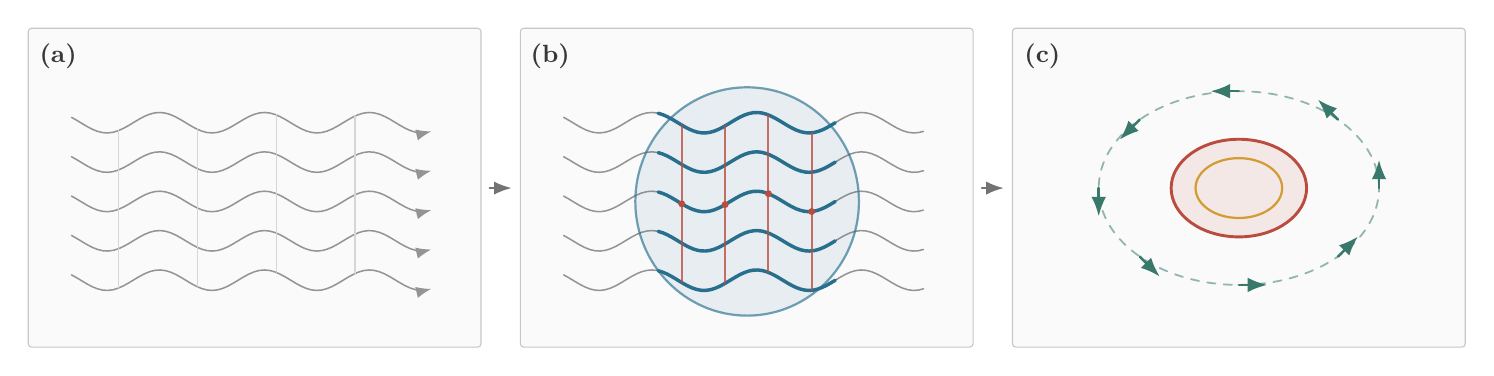
\begin{tikzpicture}[
  >=Latex,
  line cap=round,
  line join=round,
  panel/.style={draw=black!22, fill=black!2, rounded corners=1.2pt},
  panelmark/.style={font=\bfseries\small, text=black!78},
  substrate/.style={draw=black!42, line width=0.55pt},
  active/.style={draw=tefblue, line width=1.25pt},
  phase/.style={draw=tefred, line width=0.75pt},
  flow/.style={-Latex, draw=black!55, line width=0.75pt}
]
\definecolor{tefblue}{HTML}{286F8E}
\definecolor{tefred}{HTML}{B94B3F}
\definecolor{tefgold}{HTML}{D39B32}
\definecolor{tefgreen}{HTML}{39796B}

% Panel A: the realized substrate is an ensemble of rollout helices.
\begin{scope}
  \path[panel] (0,0) rectangle (5.75,4.05);
  \node[panelmark] at (0.38,3.70) {(a)};
  \foreach \y in {0.85,1.35,1.85,2.35,2.85}{
    \draw[substrate,-Latex]
      plot[domain=0.55:5.12,samples=70]
      (\x,{\y+0.13*sin(270*\x)});
  }
  \foreach \x in {1.15,2.15,3.15,4.15}{
    \draw[black!16, line width=0.45pt]
      (\x,{0.85+0.13*sin(270*\x)}) --
      (\x,{2.85+0.13*sin(270*\x)});
  }
\end{scope}

% Panel B: a localized mode has coherent support on several helices.
\begin{scope}[xshift=6.25cm]
  \path[panel] (0,0) rectangle (5.75,4.05);
  \node[panelmark] at (0.38,3.70) {(b)};
  \foreach \y in {0.85,1.35,1.85,2.35,2.85}{
    \draw[substrate]
      plot[domain=0.55:5.12,samples=70]
      (\x,{\y+0.13*sin(270*\x)});
    \draw[active]
      plot[domain=1.75:4.00,samples=42]
      (\x,{\y+0.13*sin(270*\x)});
  }
  \fill[tefblue, opacity=0.09] (2.88,1.85) ellipse (1.42 and 1.45);
  \draw[tefblue, opacity=0.65, line width=0.8pt]
    (2.88,1.85) ellipse (1.42 and 1.45);
  \foreach \x in {2.05,2.60,3.15,3.70}{
    \draw[phase, opacity=0.78]
      (\x,{0.85+0.13*sin(270*\x)}) --
      (\x,{2.85+0.13*sin(270*\x)});
    \fill[tefred] (\x,{1.85+0.13*sin(270*\x)}) circle (1.25pt);
  }
\end{scope}

% Panel C: the charged core couples to an independent degree-one texture.
\begin{scope}[xshift=12.50cm]
  \path[panel] (0,0) rectangle (5.75,4.05);
  \node[panelmark] at (0.38,3.70) {(c)};
  \fill[tefred, opacity=0.10] (2.875,2.02) ellipse (0.86 and 0.62);
  \draw[tefred, line width=1.05pt] (2.875,2.02) ellipse (0.86 and 0.62);
  \draw[tefgold, line width=0.8pt] (2.875,2.02) ellipse (0.55 and 0.38);
  \draw[tefgreen!55, dashed, line width=0.65pt]
    (2.875,2.02) ellipse (1.78 and 1.23);
  \foreach \a in {0,45,...,315}{
    \draw[-Latex, tefgreen, line width=0.9pt]
      ({2.875+1.78*cos(\a)},{2.02+1.23*sin(\a)}) --
      ({2.875+1.78*cos(\a)+0.36*cos(\a+90)},
       {2.02+1.23*sin(\a)+0.36*sin(\a+90)});
  }
\end{scope}

\draw[flow] (5.86,2.02)--(6.14,2.02);
\draw[flow] (12.11,2.02)--(12.39,2.02);
\end{tikzpicture}%
}
\caption{\textit{Schematic hierarchy of the TEF electron-like excitation. (a) The realized spacetime substrate $\Gamma_S=\{\gamma_\alpha\}$ is a source-local ensemble of neighboring rollout helices, not a single curve. (b) The charged collective field $z(x)$ represents a localized phase-coherent resonance supported across several helices, not a point on one helix or a classical ball. (c) The candidate electron-like state couples that charged core to an independent degree-one rollout-frame texture $\mathcal R$. As established later in the reduced configuration space, its spatial-rotation orbit gives a noncontractible $2\pi$ loop and a contractible twice-traversed $4\pi$ loop. The drawing is conceptual, not a microscopic derivation or a metric reconstruction.}}
\label{fig:electron-excitation-hierarchy}
\end{figure*}

\section{Unified Effective Theory}

\subsection{Gauge normalization}

Let \(n\in\mathbb Z\) be the local representation weight and \(\zeta\) the effective gauge coupling. We use
\begin{equation}
\boxed{
D_\mu z
=
(\partial_\mu+i n\zeta A_\mu)z,
}
\end{equation}
with gauge transformations
\begin{align}
z&\mapsto e^{-in\zeta\Lambda}z,\\
A_\mu&\mapsto A_\mu+\partial_\mu\Lambda.
\end{align}
The fundamental dimensionless compact angle is
\begin{equation}
\alpha=\zeta\Lambda
\pmod{2\pi}.
\end{equation}

The Maxwell kinetic term is canonical:
\begin{equation}
\mathcal L_{\rm EM}
=
-\frac14F_{\mu\nu}F^{\mu\nu},
\qquad
F_{\mu\nu}
=
\partial_\mu A_\nu-\partial_\nu A_\mu.
\end{equation}

\subsection{Scalar and frame sectors}

The scalar potential is
\begin{equation}
U(r)
=
\frac12\Omega_0^2r^2
-
\frac{\lambda}{4}r^4
+
\frac{g_6}{6}r^6,
\qquad
\lambda>0,\quad g_6>0.
\end{equation}

For the rollout-frame field define
\begin{equation}
\boxed{
L_\mu
=
\mathcal R^{-1}\partial_\mu\mathcal R
\in\mathfrak{so}(3).
}
\end{equation}
Because \(\mathcal R\) is an internal group-valued spacetime scalar in the present effective model, \(\partial_\mu\) acts only on its spacetime dependence. No additional physical-frame tensor index or background spin connection acts on \(\mathcal R\) in this paper. A more microscopic rollout-frame covariant derivative would be a later refinement rather than an implicit ingredient of the present action.

To avoid representation-dependent trace factors, we normalize the invariant Lie-algebra inner product by
\begin{equation}
\boxed{
\langle X,Y\rangle
=
-\frac12\operatorname{tr}_{2}
(\widetilde X\widetilde Y)
=
-\frac18\operatorname{tr}_{3}(XY),
}
\end{equation}
where \(\widetilde X,\widetilde Y\in\mathfrak{su}(2)\) are corresponding lifted algebra elements.

The frame Lagrangian is
\begin{equation}
\boxed{
\mathcal L_R
=
\frac{A(|z|^2)}{2}
\langle L_\mu,L^\mu\rangle
-
\frac{B}{16}
\langle
[L_\mu,L_\nu],
[L^\mu,L^\nu]
\rangle.
}
\end{equation}

The scalar-dependent frame stiffness is chosen as
\begin{equation}
\boxed{
A(|z|^2)
=
A_0
-
\chi
\frac{|z|^2}{z_0^2+|z|^2},
}
\end{equation}
with
\begin{equation}
A_0>\chi>0,
\qquad
z_0>0,
\qquad
B>0.
\end{equation}
This bounded softening provides a direct energetic mechanism by which a localized charged core can favor overlap with a nontrivial frame texture while keeping the frame stiffness positive.

\subsection{Master action}

The unified effective action is
\begin{equation}
\boxed{
\begin{aligned}
S_{\rm eff}
&=
\int d^4x\,\sqrt{-g_{\rm roll}}\\
&\quad\times
\left[
-\frac14F_{\mu\nu}F^{\mu\nu}
+\frac12(D_\mu z)^\ast D^\mu z
\right.\\[-0.2em]
&\qquad\left.
-U(|z|)+\mathcal L_R
\right].
\end{aligned}
}
\end{equation}

This action is an effective compatibility model. The quartic--sextic scalar potential and the bounded frame-softening function are test structures, not yet derived from primitive multi-helix dynamics.

\subsection{Boundary sector}

For the one-excitation topology calculation we restrict the spatial domain to
\begin{equation}
\Sigma\simeq\mathbb R^3
\end{equation}
with one asymptotic end. The metric may be treated more generally in principle, but the explicit U1 solution and the spin orbit studied below use the flat effective background.

We select the based vacuum sector
\begin{align}
z(x)&\to0,\\
A_i(x)&\to0
\quad\text{in the chosen asymptotic gauge},\\
\mathcal R(x)&\to I,
\qquad
(|x|\to\infty).
\end{align}

The last condition is a boundary-sector choice, not a consequence of finite derivative energy alone.

\section{A Joint Stationary Charged--Textured Solution}

\subsection{Flat-background radial ansatz}

The explicit joint calculation is performed on
\begin{equation}
\boxed{
\mathfrak B_0
=
(\mathbb R^3,\delta_{ij},e^a{}_i=\delta^a{}_i,\ldots).
}
\end{equation}

We use
\begin{equation}
z(r,t)
=
u(r)e^{-i\omega t},
\qquad
A_0=\phi(r),
\qquad
A_i=0,
\end{equation}
and a degree-one \(SU(2)\) lift of the rollout-frame texture,
\begin{equation}
g_R(r)
=
\cos f(r)
+
i\hat{\bm x}\cdot\bm\sigma\,\sin f(r).
\end{equation}

Define
\begin{equation}
\Omega(r)
=
\omega-\zeta\phi(r),
\end{equation}
and
\begin{equation}
A(u^2)
=
A_0-\chi\frac{u^2}{z_0^2+u^2}.
\end{equation}

For the numerical example,
\begin{equation}
\Omega_0=1,\quad
\lambda=2,\quad
g_6=1,
\end{equation}
\begin{equation}
A_0=1,\quad
B=2,\quad
\chi=0.35,\quad
z_0=1,
\end{equation}
and
\begin{equation}
\omega=0.8,
\qquad
\zeta=0.10.
\end{equation}

\subsection{Reduced field equations}

Let
\begin{equation}
e_2
=
f'^2
+
\frac{2\sin^2f}{r^2},
\end{equation}
\begin{equation}
e_4
=
\frac{2\sin^2f\,f'^2}{r^2}
+
\frac{\sin^4f}{r^4},
\end{equation}
and
\begin{equation}
A_u
=
-\frac{2\chi z_0^2u}{(z_0^2+u^2)^2}.
\end{equation}

The coupled radial equations are
\begin{equation}
\boxed{
u''
+
\frac{2}{r}u'
=
(\Omega_0^2-\Omega^2)u
-
\lambda u^3
+
g_6u^5
+
\frac12A_u e_2,
}
\end{equation}
\begin{equation}
\boxed{
\phi''
+
\frac{2}{r}\phi'
=
-\zeta\Omega u^2,
}
\end{equation}
and
\begin{equation}
\boxed{
\begin{aligned}
f''={}&\frac{1}{r^2A+2B\sin^2 f}\Bigl[
2A\sin f\cos f
\\
&-2B\sin f\cos f\,f'^2
+\frac{2B\sin^3 f\cos f}{r^2}
\\
&-2rAf'-r^2A_u u'f'
\Bigr].
\end{aligned}
}
\end{equation}

The continuum regularity and outer boundary conditions are
\begin{align}
u'(0)&=0,
&
\phi'(0)&=0,
&
f(0)&=\pi,
\\
u(R)&=0,
&
\phi(R)&=0,
&
f(R)&=0.
\end{align}

The implemented numerical solve starts at
\begin{equation}
r_{\min}=10^{-3}
\end{equation}
rather than evaluating singular radial coefficients at the origin. Numerical details are collected in Appendix~\ref{app:numerics}.

\subsection{Energy and charge normalization}

For the numerical U1 branch we take the local representation weight \(n=1\). It is useful to distinguish three charge notions from the outset:
\begin{equation}
\boxed{
\mathcal N
=
4\pi\int_0^R r^2\Omega u^2\,dr
}
\end{equation}
is the normalized classical phase/Noether charge carried by the matter profile;
\begin{equation}
\boxed{
\mathcal Q_{\rm M}^{\rm(cl)}
=
\zeta\mathcal N
=
-4\pi[r^2\phi']_0^R
}
\end{equation}
is the corresponding classical Maxwell source/flux in the canonical gauge-field normalization used here; and the later quantum physical charge is denoted
\begin{equation}
Q_{\rm phys}=k e_*.
\end{equation}
The numerical value \(82.382379\) quoted below is \(\mathcal N\), not \(Q_{\rm phys}\).

The stationary radial functional is
\begin{equation}
\begin{aligned}
\mathcal I_\omega
={}&4\pi\int_0^R r^2\Bigl[
\tfrac12\Omega^2u^2-\tfrac12u'^2-U(u)
\\
&\hspace{3.5em}
+\tfrac12\phi'^2-\tfrac12(Ae_2+B e_4)
\Bigr]dr.
\end{aligned}
\end{equation}

The energy is
\begin{equation}
\boxed{
\begin{aligned}
E
={}&4\pi\int_0^R r^2\Bigl[
\tfrac12\Omega^2u^2+\tfrac12u'^2+U(u)
\\
&\hspace{3.5em}
+\tfrac12\phi'^2+\tfrac12(Ae_2+B e_4)
\Bigr]dr.
\end{aligned}
}
\end{equation}


\subsection{Numerical solution}

On the primary box
\begin{equation}
R=40,
\end{equation}
the coupled boundary-value problem converges to
\begin{align}
\mathcal N
&\simeq
82.382379,
\\
E
&\simeq
174.450853,
\\
u(0)
&\simeq
1.320297,
\\
\phi(0)
&\simeq
0.330348.
\end{align}

The central frame stiffness is
\begin{equation}
A(0)\simeq0.777589,
\end{equation}
and remains positive.

The radial boundary conditions select the degree-one hedgehog sector. Numerical integration gives
\begin{equation}
\nu\simeq0.999999998,
\end{equation}
which is used as a consistency check on the implementation rather than as an independent dynamical no-unwinding test.

The canonical reproduction run has
\begin{equation}
\text{Gauss relative mismatch}
\simeq1.55\times10^{-10},
\end{equation}
and maximum BVP rms residual
\begin{equation}
\simeq9.94\times10^{-7}.
\end{equation}

Figure~\ref{fig:jointprofiles} shows the simultaneous scalar, electrostatic, and texture profiles.

\begin{figure}[ht]
\centering
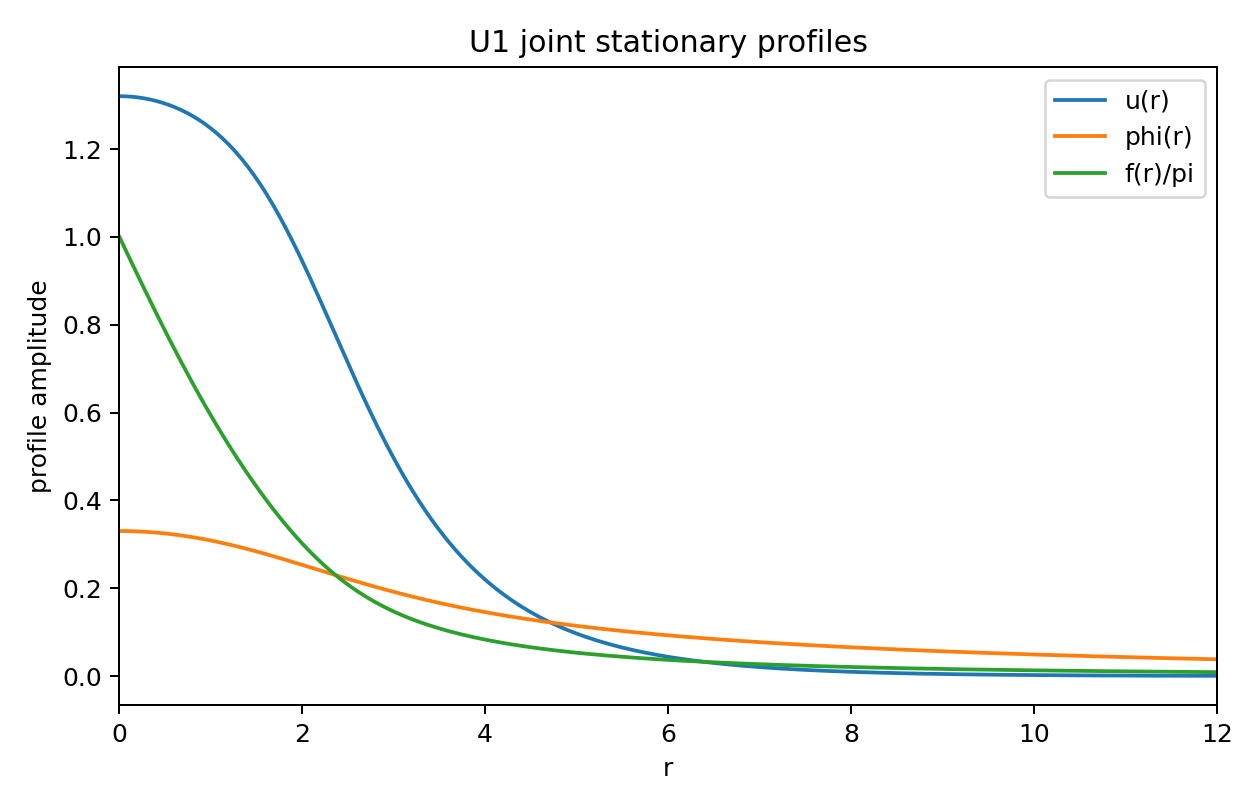
\includegraphics[width=0.78\linewidth]{TEF_U1_joint_profiles_v0.4.png}
\caption{Joint stationary profiles on the \(R=40\) box: scalar amplitude \(u(r)\), electrostatic potential \(\phi(r)\), and normalized frame angle \(f(r)/\pi\).}
\label{fig:jointprofiles}
\end{figure}

The same branch was followed over
\begin{equation}
R=12,16,20,24,32,40.
\end{equation}
The localized core observables vary smoothly, while \(\mathcal N\) and \(E\) show the expected finite-box drift associated with the long-range electrostatic tail. The solver/grid and origin-cutoff checks are reported in Appendix~\ref{app:numerics}.

\subsection{Finite-box reference-channel energetics}

To test whether the joint solution is energetically preferred over a simple factorized reference, we define at each outer radius \(R\)
\begin{equation}
\boxed{
\Delta E_{\rm ref}^{(R)}
=
E_{\rm core}^{\rm iso}(R,\mathcal N)
+
E_{R}^{\rm iso}(R)
-
E_{\rm joint}(R,\mathcal N).
}
\end{equation}

The two isolated terms are solved separately as centered one-body boundary-value problems. This is not the energy of two resolved objects displaced to large separation inside one common finite ball, and it is not identified with the exact infinite-domain dissociation threshold.

At \(R=40\),
\begin{align}
E_R^{\rm iso}
&\simeq
103.134600383,
\\
E_{\rm core}^{\rm iso}
&\simeq
79.203348055,
\\
E_{\rm ref}^{(40)}
&\simeq
182.337948438.
\end{align}
Therefore
\begin{equation}
\boxed{
\Delta E_{\rm ref}^{(40)}
\simeq
7.887095517
>
0.
}
\end{equation}

Repeating the reference construction gives
\begin{center}
\begin{tabular}{rrrr}
\toprule
\(R\) & \(E_{\rm joint}\) & \(E_{\rm ref}^{(R)}\) & \(\Delta E_{\rm ref}^{(R)}\)\\
\midrule
20 & 172.640290 & 180.443019 & 7.802729\\
24 & 173.216746 & 181.046617 & 7.829871\\
32 & 173.975542 & 181.840714 & 7.865172\\
40 & 174.450853 & 182.337948 & 7.887096\\
\bottomrule
\end{tabular}
\end{center}

A diagnostic linear fit in \(1/R\) gives
\begin{equation}
\Delta E_{\rm ref}^{(\infty)}
\simeq
7.970992.
\end{equation}
This extrapolation only estimates finite-box sensitivity of the reference sum; it is not promoted to a rigorous continuum dissociation threshold.

The result established by this section is therefore:
\begin{equation}
\boxed{
\begin{minipage}{0.84\linewidth}
The unified effective theory admits one explicit stationary object in which a charged nonlinear core, its self-consistent electrostatic field, and a degree-one rollout-frame texture coexist with mutual backreaction.
\end{minipage}
}
\end{equation}

\section{Configuration-Space Spin Topology of a U1-Associated Full-Space Representative}

\subsection{From the finite-box stationary solution to a full-space spatial representative}

The numerical U1 boundary-value problem produces
\begin{equation}
\Phi_\star^{(R)}
=
\bigl(
z_\star^{(R)},
A_{\star0}^{(R)},
\mathcal R_\star^{(R)}
\bigr)
\end{equation}
only on the truncated radial interval
\begin{equation}
r_{\min}\le r\le R,
\qquad
r_{\min}=10^{-3},
\qquad
R=40.
\end{equation}
It is therefore not literally an element of a smooth full-space configuration space on \(\mathbb R^3\).

The finite-box sequence and cutoff-convergence tests support the interpretation of the U1 branch as localized, but no rigorous infinite-domain stationary-solution theorem is claimed. The topology argument requires less: a smooth finite-energy spatial representative in the same degree-one texture sector and constructed directly from the finite-box scalar and texture profiles.

Choose narrow inner and outer collars,
\begin{equation}
\begin{gathered}
0<r<2r_{\min},
\qquad
R-\delta<r<R+\delta,
\\
0<\delta\ll R.
\end{gathered}
\end{equation}

For the scalar amplitude, the inner completion is chosen so that in a neighborhood of the origin
\begin{equation}
\boxed{
\widetilde u(r)=U(r^2)
}
\end{equation}
for some smooth function \(U\). This is the ordinary three-dimensional radial smoothness condition: all odd radial derivatives vanish at \(r=0\), not merely the first derivative.

For the degree-one hedgehog texture,
\begin{equation}
\widetilde g_R
=
\cos\widetilde f
+
i\hat{\bm x}\cdot\bm\sigma\,
\sin\widetilde f,
\end{equation}
the inner completion is chosen in the form
\begin{equation}
\boxed{
\widetilde f(r)
=
\pi-r\,H(r^2)
}
\end{equation}
with \(H\) smooth near \(r=0\). Then
\begin{equation}
\frac{\sin\widetilde f(r)}{r}
\end{equation}
is a smooth function of \(r^2\), so
\begin{equation}
\hat{\bm x}\sin\widetilde f(r)
=
\bm x\,
\frac{\sin\widetilde f(r)}{r}
\end{equation}
extends smoothly through the origin. Thus ``\(C^\infty\) completion'' in this paper means smoothness of the resulting three-dimensional fields, not merely smoothness of radial functions on the half-line.

The inner completion is matched smoothly to the numerical profiles by \(r=2r_{\min}\). In the outer collar the scalar amplitude and texture are smoothly taken to their vacuum values and remain there for \(r\ge R+\delta\):
\begin{equation}
\widetilde u(r)=0,
\qquad
\widetilde f(r)=0.
\end{equation}

Consequently, on the prescribed bulk interval
\begin{equation}
\boxed{
2r_{\min}\le r\le R-\delta,
}
\end{equation}
the relations
\begin{equation}
\boxed{
\widetilde u(r)=u_\star^{(R)}(r),
\qquad
\widetilde f(r)=f_\star^{(R)}(r)
}
\end{equation}
are exact by construction.

No corresponding exact statement is made for the electrostatic potential or the gauge-invariant frequency. If an electrostatic full-space completion is desired, one may solve
\begin{equation}
\widetilde\phi''
+
\frac2r\widetilde\phi'
=
-\zeta
\bigl(
\widetilde\omega-\zeta\widetilde\phi
\bigr)
\widetilde u^2
\end{equation}
with
\begin{equation}
\widetilde\phi'(0)=0,
\qquad
\widetilde\phi(\infty)=0.
\end{equation}
Outside the completed matter support it then has the Coulomb form
\begin{equation}
\widetilde\phi(r)=\frac{\widetilde C}{r}.
\end{equation}
Because the matter profile has been modified in the collars and Gauss law is solved globally, neither
\begin{equation}
\widetilde\phi(r)=\phi_\star^{(R)}(r)
\end{equation}
nor
\begin{equation}
\widetilde\Omega(r)
=
\widetilde\omega-\zeta\widetilde\phi(r)
=
\omega-\zeta\phi_\star^{(R)}(r)
\end{equation}
is asserted on the bulk. No quantitative electrostatic matching error is used in the topology proof.

The reduced spatial configuration representative used below is therefore
\begin{equation}
\boxed{
\widetilde X_\star^{(R)}
=
\bigl(
\widetilde z_\star^{(R)},
\widetilde A_{\star i}^{(R)}=0,
\widetilde{\mathcal R}_\star^{(R)}
\bigr).
}
\end{equation}

The two objects have different evidential roles:
\begin{equation}
\boxed{
\Phi_\star^{(R)}
=
\text{finite-box stationary numerical solution},
}
\end{equation}
with the quoted \(\mathcal N\), energy, Gauss closure, and finite-box reference energetics, whereas
\begin{equation}
\boxed{
\begin{aligned}
\widetilde X_\star^{(R)}
&=\text{smooth full-space spatial}
\\
&\quad\text{configuration representative used}
\\
&\quad\text{in the topology proof}
\end{aligned}
}
\end{equation}

No numerical value of the full-space representative's charge or energy is identified with the finite-box values. The scalar/frame collar completion is also not claimed to satisfy their stationary Euler--Lagrange equations in the gluing regions. The construction provides a topology basepoint, not a second stationary-solution calculation.

\subsection{Physical reduced configuration space}

For the topology argument, let
\begin{equation}
\mathscr F_1^\infty(\mathfrak B_0)
\end{equation}
be the smooth finite-energy degree-one \emph{spatial} field sector
\begin{equation}
(z,A_i,\mathcal R)
\end{equation}
on the same flat background, with the selected asymptotic conditions
\begin{align}
z(x)&\to0,\\
A_i(x)&\to0,\\
\mathcal R(x)&\to I.
\end{align}
The temporal potential \(A_0\) is not an independent coordinate of this reduced spatial quotient. A Gauss-law electrostatic completion may be associated with a stationary representative when needed, but the homotopy argument below depends only on the spatial fields \((z,A_i,\mathcal R)\).

The texture is required to extend continuously to the one-point compactification:
\begin{equation}
\overline{\mathcal R}
\in
C_*^0(S^3,SO(3)),
\qquad
\overline{\mathcal R}(\infty)=I.
\end{equation}

We equip the physical field space with a topology generated by local \(C^1\) convergence on compact subsets, convergence of the finite-energy seminorms appearing in the effective action, and uniform convergence of the compactified texture map.

The gauge group is
\begin{equation}
\mathcal G_0^\infty
=
\left\{
\begin{aligned}
&\Lambda\in C^\infty(\mathbb R^3,\mathbb R):
\\[-1mm]
&\Lambda(x)\to0,
\quad\partial_i\Lambda(x)\to0,
\\[-1mm]
&d\Lambda\in L^2
\end{aligned}
\right\},
\end{equation}
acting by
\begin{align}
z&\mapsto e^{-in\zeta\Lambda}z,\\
A_i&\mapsto A_i+\partial_i\Lambda,\\
\mathcal R&\mapsto\mathcal R.
\end{align}

The pointwise decay condition on \(\partial_i\Lambda\) is imposed so that a gauge transformation preserves the selected asymptotic condition \(A_i\to0\). The definition is intentionally stronger than a minimal Sobolev condition; no claim of functional-analytic optimality is needed here.

The reduced one-excitation space is
\begin{equation}
\boxed{
\mathscr C_1(\mathfrak B_0)
=
\mathscr F_1^\infty(\mathfrak B_0)
/\mathcal G_0^\infty.
}
\end{equation}

Because the gauge group acts trivially on \(\mathcal R\), the texture forgetful map descends continuously to
\begin{equation}
\boxed{
P_R:
\mathscr C_1(\mathfrak B_0)
\longrightarrow
C_*^0(S^3,SO(3))_1.
}
\end{equation}

No equality or homotopy equivalence between the full physical field space and the ambient continuous texture mapping space is assumed.

\subsection{The spin map based at the U1-associated full-space representative}

Let
\begin{equation}
\widetilde X_\star^{(R)}
=
(\widetilde z_\star,0,\widetilde{\mathcal R}_\star)
\in
\mathscr F_1^\infty(\mathfrak B_0)
\end{equation}
denote the smooth full-space spatial representative constructed above from the finite-box U1 scalar and texture profiles.

For each
\begin{equation}
S\in SO(3),
\end{equation}
define the active rotation on the fixed background by
\begin{align}
z^S(x,t)
&=
z(S^{-1}x,t),
\\
A^S
&=
(S^{-1})^\ast A,
\\
\mathcal R^S(x)
&=
\mathcal R(S^{-1}x).
\end{align}

This gives a continuous orbit map
\begin{equation}
\boxed{
\begin{aligned}
f_{\rm spin}^{\rm joint}:\quad
SO(3)&\longrightarrow\mathscr C_1(\mathfrak B_0),
\\
S&\longmapsto[S\cdot\widetilde X_\star^{(R)}].
\end{aligned}
}
\end{equation}

Its basepoint is the full-space representative constructed from the numerical U1 scalar and texture profiles:
\begin{equation}
\boxed{
f_{\rm spin}^{\rm joint}(I)
=
[\widetilde X_\star^{(R)}].
}
\end{equation}

Because the completed scalar amplitude is radial and \(\widetilde A_{\star i}=0\),
\begin{equation}
f_{\rm spin}^{\rm joint}(S)
=
\left[
\widetilde z_\star,\,
0,\,
\widetilde{\mathcal R}_\star(S^{-1}x)
\right].
\end{equation}
Thus only the texture traces a nonconstant orbit in the reduced spatial configuration space. Boundary conditions, three-dimensional smoothness, and finite energy are preserved along the orbit. The topology conclusion does not require the representative to remain an exact stationary solution.

\subsection{The \texorpdfstring{\(2\pi\)}{2pi} loop}

The topology theorem is applied to
\begin{equation}
\mathcal M_1
=
C_*^0(S^3,SO(3))_1.
\end{equation}

Because the compactified domain is \(S^3\), every based texture has a unique based lift
\begin{equation}
g:S^3\to SU(2)\simeq S^3.
\end{equation}
The lift preserves the integer degree.

For the actual spin orbit,
\begin{equation}
P_R\circ
f_{\rm spin}^{\rm joint}(S)
=
\overline{\widetilde{\mathcal R}_\star(S^{-1}x)}.
\end{equation}
This is the standard spatial-precomposition orbit of a degree-one based map.

The Giulini/Krusch parity theorem gives
\begin{equation}
\boxed{
[\gamma_{2\pi}^{R}]
=
1
\in
\pi_1(\mathcal M_1)
\simeq
\mathbb Z_2
}
\end{equation}
for odd degree \cite{Giulini1993,Krusch2003,Krusch2006}.

If the full joint loop were contractible in \(\mathscr C_1(\mathfrak B_0)\), applying the continuous projection \(P_R\) to the contraction would contract \(\gamma_{2\pi}^{R}\) in \(\mathcal M_1\), a contradiction. Therefore
\begin{equation}
\boxed{
[\gamma_{2\pi}^{\rm joint}]
\neq0.
}
\end{equation}

\subsection{The \texorpdfstring{\(4\pi\)}{4pi} loop}

The full spin map is defined on all of \(SO(3)\). The twice-traversed rotation loop satisfies
\begin{equation}
[4\pi]
=
0
\in
\pi_1(SO(3)).
\end{equation}

Let
\begin{equation}
H:D^2\to SO(3)
\end{equation}
be a contraction. Then
\begin{equation}
f_{\rm spin}^{\rm joint}\circ H
\end{equation}
is a contraction of the full \(4\pi\) loop in the joint configuration space. Hence
\begin{equation}
\boxed{
2\pi\ {\rm noncontractible},
\qquad
4\pi\ {\rm contractible}.
}
\end{equation}

Pontryagin--Thom framing provides a useful geometric interpretation of the local orientational content of the degree-one texture, but it is not required as an intermediate representative in this proof \cite{Sorkin1988,AucklySpeight2006}.

\subsection{Scope: spin topology, not angular-momentum dynamics}

The word ``spin'' in this section refers to the topology of the framed one-excitation configuration space.

The result does not derive a Noether or quantum angular-momentum operator, a rotational collective-coordinate Lagrangian, a normalizable rotational zero mode, a moment of inertia, or a rotational spectrum.

For the actual U1 calculation the background and effective action are rotationally invariant, so the \(SO(3)\) orbit is well defined. The proof uses only continuity of that orbit and the topology of the configuration space.

\section{Toward Identification with the Physical Electron}

The preceding sections establish one charged-textured object with spinorial configuration topology. They do not yet complete the physical identification with the observed electron.

\subsection{Finkelstein--Rubinstein representation}

The nontrivial \(2\pi\) loop permits the nontrivial one-dimensional FR representation
\begin{equation}
\rho_{\rm FR}(1)=-1.
\end{equation}
If selected,
\begin{equation}
\Psi(2\pi)=-\Psi,
\qquad
\Psi(4\pi)=+\Psi.
\end{equation}

Topology makes this spinorial quantization available; it does not by itself force Nature to select the nontrivial representation. Nor does the \(\mathbb Z_2\) loop alone select
\begin{equation}
j=\frac12
\end{equation}
over higher half-integer representations.

The two-object exchange loop remains a separate TEF construction. General FR/Sorkin theory motivates the relation between rotation and exchange \cite{Sorkin1988,AucklySpeight2006}, but it is not substituted here for a TEF-specific two-excitation calculation.

\subsection{Residual electric-charge sectors}

Gauge transformations trivial at infinity are redundancies. Transformations approaching a constant define a residual compact group
\begin{equation}
U(1)_\infty.
\end{equation}

A quantum state in a fixed total-charge sector transforms as
\begin{equation}
\boxed{
\Psi
\mapsto
e^{ik\alpha_\infty}\Psi,
\qquad
k\in\mathbb Z.
}
\end{equation}

Once the physical normalization \(e_*\) of the compact connection is fixed,
\begin{equation}
\boxed{
Q_{\rm phys}=k e_*.
}
\end{equation}

The classical U1 branch is labeled by the continuous normalized phase charge \(\mathcal N(\omega)\), while its classical Maxwell source/flux is \(\mathcal Q_{\rm M}^{\rm(cl)}=\zeta\mathcal N\). A future quantization must relate this semiclassical branch to a quantum residual-charge sector, in particular to a candidate \(k=\pm1\) state. This identification is not assumed in the present numerical calculation.

\subsection{\texorpdfstring{\(\operatorname{Spin}^c\)}{Spin-c} compatibility}

A stronger effective possibility is
\begin{equation}
\operatorname{Spin}^c(3)
=
\frac{SU(2)\times U(1)}{\mathbb Z_2}
\simeq
U(2)
\end{equation}
\cite{Nicolaescu2000}.

If the \(U(1)\) factor is the same normalized electromagnetic \(U(1)_\infty\), then a spin-\(j\) state with total electromagnetic weight \(k\) obeys
\begin{equation}
\boxed{
2j+k=0\pmod2.
}
\end{equation}
Thus a half-integer spin representation would require odd electromagnetic weight. The central gluing remains an effective structural hypothesis rather than a result derived from primitive rollout transport.

\subsection{Dirac closure as the next dynamical target}

Spinorial configuration topology does not derive a four-component Dirac equation.

The next low-energy question is whether collective quantization of the actual charged-textured solution reduces to a first-order operator of the form
\begin{equation}
\mathcal D_{\rm eff}
=
i\hbar c\gamma^a e_a{}^\mu D_\mu
-
E_0.
\end{equation}

If such a closure is obtained, it would naturally imply
\begin{equation}
E^2
=
E_0^2+c^2P^2
\end{equation}
and would place the excitation and electromagnetic sectors on the same characteristic cone.

Minimal Dirac coupling would also give the leading weak-field magnetic relation
\begin{equation}
g=2,
\end{equation}
but this is a benchmark consequence of a future Dirac-type closure, not a result already derived here. Symmetry-allowed Pauli terms may modify the conclusion unless their coefficients are microscopically controlled.

\subsection{Evidence status}

The current status can be summarized as follows:

\begin{table*}[t]
\centering
\small
\caption{Current evidence status and the corresponding open requirements.}
\label{tab:evidence-status}
\begin{tabular}{p{0.16\textwidth}p{0.37\textwidth}p{0.37\textwidth}}
\toprule
\textbf{Question} & \textbf{Established here} & \textbf{Still open}\\
\midrule
Joint object &
One stationary charged core, electrostatic field, and degree-one frame texture in one coupled solution &
Full nonspherical spectral/nonlinear stability; moving full composite
\\[1mm]
Energetics &
Positive matched-charge finite-box reference-channel gap &
Same-box two-center separation energy; exact infinite-domain dissociation threshold
\\[1mm]
Spin topology &
U1-associated smooth full-space representative has noncontractible \(2\pi\) and contractible \(4\pi\) configuration-space loops &
FR-sign selection; \(j=1/2\); dynamical angular-momentum spectrum
\\[1mm]
Electric charge &
Residual compact sectors labeled by \(k\in\mathbb Z\); classical \(\mathcal N\) and Maxwell flux \(\zeta\mathcal N\) distinguished &
Identification of the U1 quantum state with \(k=\pm1\) and the observed electron charge
\\[1mm]
Statistics &
FR-compatible spinorial sector is available &
TEF-specific two-object exchange loop
\\[1mm]
Low-energy dynamics &
A Dirac-type closure target is defined &
Derivation of the Dirac operator, \(g=2\), radiative corrections, QED
\\
\bottomrule
\end{tabular}
\end{table*}

\section{Relation to Existing Soliton and Spinorial-Quantization Theory}

The scalar core belongs to the broad family of non-topological soliton constructions initiated by Q-balls \cite{Coleman1985}. Gauged Q-ball theory provides a mature comparison class, including sixth-order potentials of the same broad type used here \cite{Lee1989,HanSu2023}. Long-range gauge repulsion is known to restrict gauged-Q-ball branches and can produce maximal charge or size \cite{HeeckZhi2026}. The present U1 result is therefore not a claim that gauged localization exists for arbitrary coupling or charge.

Gauged Q-balls can also possess nonspherical instabilities that are invisible to a purely radial existence calculation \cite{Rajaraman2025}. This is why the present paper distinguishes stationary radial existence from full three-dimensional orbital stability.

A neighboring construction couples a topological matter field directly to electromagnetism. Electrically charged degree-one gauged Skyrmions with Maxwell fields, magnetic flux, dipole moments, and angular momentum have been constructed explicitly \cite{Livramento2023}. The TEF effective construction factorizes these roles differently:
\begin{equation}
\boxed{
\begin{aligned}
z&=\text{non-topological charged resonance},
\\
\mathcal R&=\text{independent rollout-frame topology}.
\end{aligned}
}
\end{equation}
The main U1 question is whether these independent sectors can form one self-consistent object.

The configuration-space topology used in Section 5 is standard FR/Skyrmion mathematics \cite{Giulini1993,Krusch2003,Krusch2006,CorkHarland2024}. The research claim is not the discovery of the \(\mathbb Z_2\) loop itself. The TEF-specific construction has two linked parts: the unified effective action yields a finite-box stationary charged-textured U1 solution, and a smooth full-space spatial representative built from its scalar and degree-one texture profiles projects to the same odd-degree based mapping-space sector. The latter is a configuration-space representative, not an independently solved full-space stationary solution.

Another neighboring line introduces an explicit Dirac fermion field localized on a gauged-Q-ball background \cite{Dzhunushaliev2025}. TEF aims at a different closure: the spinorial low-energy variable should emerge from collective quantization of the charged-textured composite itself rather than being added as an independent fermionic field.

\section{Discussion and Conclusion}

The previous TEF electromagnetic paper addressed the low-energy gauge field. The present paper addresses the electron-like matter sector that couples to it.

The result is not a first-principles electron derivation. It is nevertheless stronger than a collection of analogies. One normalized effective action contains the collective charged mode, the electromagnetic connection, and the rollout-frame texture. On the finite numerical domain that action admits one explicit stationary radial solution in which all three coexist with mutual backreaction. Separately, a smooth full-space spatial representative constructed from the finite-box scalar and texture profiles lies in a degree-one frame-texture sector whose \(SO(3)\) orbit has
\begin{equation}
\boxed{
2\pi\ {\rm noncontractible},
\qquad
4\pi\ {\rm contractible}.
}
\end{equation}

At the effective compatibility level, the two linked constructions therefore show that the same effective model supports
\begin{equation}
\boxed{
\begin{gathered}
\text{a stationary finite-box}
\\
\text{charged-textured solution}
\end{gathered}
}
\end{equation}
and
\begin{equation}
\boxed{
\begin{gathered}
\text{an associated degree-one representative}
\\
\text{with spinorial rotation topology}
\end{gathered}
}
\end{equation}
The quoted finite-box \(\mathcal N\), energy, and reference-channel gap are properties of the first object and are not assigned unchanged to the second. The relation between them is constructive association through the scalar and texture profiles, not identity of all numerical or stationary properties.

That is the principal result of the paper.

Several conditions remain before the object can be identified with the physical electron. The nontrivial FR representation must be selected rather than merely allowed; \(j=1/2\) must be dynamically isolated; the classical Gauss branch must be connected to a quantum \(k=\pm1\) charge sector; the two-object exchange loop must be constructed; and the collective low-energy dynamics must reduce to an appropriate spinor equation. Only after both the electromagnetic and electron sectors are quantized as interacting fields would it be appropriate to speak of a TEF QED-like sector.

The longer-term TEF objective is more demanding still: the effective action used here should ultimately be derived from primitive multi-helix rollout dynamics rather than posited as a compatibility model. The present construction identifies a concrete target for that derivation.

\appendix

\section{Precursor Component Diagnostics}

The unified calculation was preceded by a sequence of restricted tests. They are retained here as diagnostics rather than as independent proof steps.

\subsection{Ungauged localized resonance}

For the scalar sector
\begin{equation}
\begin{aligned}
L_{\rm ex}
={}&\frac12\sum_\alpha|\dot z_\alpha|^2
-\frac{\kappa}{2}
\sum_{\langle\alpha\beta\rangle}
w_{\alpha\beta}|z_\alpha-z_\beta|^2
\\
&-\sum_\alpha U(|z_\alpha|),
\end{aligned}
\end{equation}
a stationary rotating ansatz
\begin{equation}
z_\alpha=u_\alpha e^{-i\omega t}
\end{equation}
produced localized sub-gap branches on finite graphs. On a \(C_{24}\) cycle with
\begin{equation}
\Omega_0=1,\quad
\lambda=2,\quad
g_6=1,\quad
\kappa=0.04,\quad
\omega=0.8,
\end{equation}
one representative solution had
\begin{equation}
\begin{aligned}
E&\simeq1.71428,
&|Q|&\simeq2.87195,
\\
N_{\rm eff}&\simeq2.04007.
\end{aligned}
\end{equation}
Here \(Q\) is retained only as the historical notation of that precursor diagnostic; the unified U1 sector uses \(\mathcal N\) for the normalized phase charge.

This established a localization mechanism but not an essentially multi-helix microscopic electron model.

\subsection{Electrostatic and transverse-EM diagnostics}

A finite cubic-product surrogate with self-consistent electrostatics produced a localized charged state obeying Gauss closure at numerical precision and a Coulombic far field. Constrained time evolution remained bounded over the tested finite intervals.

A separate transverse-electromagnetic calculation showed that matter perturbations source gauge-field dynamics while Coulomb-gauge constraints remain numerically controlled.

These tests motivated the electromagnetic coupling later incorporated into the joint U1 action.

\subsection{Continuum mobility diagnostic}

In a homogeneous continuum scalar limit,
\begin{equation}
\mathcal L_z
=
\frac12|\partial_t z|^2
-
\frac{c^2}{2}|\nabla z|^2
-
U(|z|),
\end{equation}
the one-dimensional profile
\begin{equation}
\begin{aligned}
u^2(x)
&=
\frac{2\delta}
{1+s\cosh(2\sqrt{\delta}\,x)},
\\
\delta&=1-\omega^2,
&s&=\sqrt{1-\frac{4\delta}{3}},
\end{aligned}
\end{equation}
at \(\omega=0.8\) has
\begin{equation}
E_0\simeq1.107737365.
\end{equation}
The boosted Lorentz-form family satisfies
\begin{equation}
E^2=E_0^2+c^2P^2.
\end{equation}

This diagnostic motivates a relativistic low-energy target but is not a moving solution of the full charged-textured U1 system.

\subsection{Early frame-texture diagnostic}

Before the fully coupled U1 calculation, a radial frame texture was tested against a prescribed localized core surrogate and showed finite-scale overlap preference. Because that surrogate did not use the final \(A(|z|^2)\) coupling, its numerical values are not used as evidence in the main text. Its role was only to motivate the joint variational problem that U1 subsequently solved.

\section{Normalization and Radial Reduction}

\label{app:normalization}

For the degree-one hedgehog lift,
\begin{equation}
e_2
=
f'^2+\frac{2\sin^2f}{r^2},
\qquad
e_4
=
\frac{2\sin^2f\,f'^2}{r^2}
+
\frac{\sin^4f}{r^4}.
\end{equation}

The invariant normalization
\begin{equation}
\langle X,Y\rangle
=
-\frac12\operatorname{tr}_2(\widetilde X\widetilde Y)
=
-\frac18\operatorname{tr}_3(XY)
\end{equation}
gives
\begin{equation}
\sum_i\langle L_i,L_i\rangle=e_2,
\end{equation}
and
\begin{equation}
\sum_{i,j}
\langle[L_i,L_j],[L_i,L_j]\rangle
=
8e_4.
\end{equation}

Hence the static frame energy is
\begin{equation}
E_R
=
4\pi
\int_0^R
r^2
\frac12
\left[
A(u^2)e_2+B e_4
\right]dr.
\end{equation}

This normalization is the one used in both the written action and the numerical solver. The scalar kinetic normalization is likewise fixed at \(1/2\), so the continuum, stationary, and time-domain equations use the same convention.

\section{Numerical Protocol and Reproducibility}

\label{app:numerics}

The primary U1 solve uses Python 3.13.5, NumPy 2.3.5, and SciPy 1.17.0. The coupled radial system is solved with
\begin{equation}
\texttt{scipy.integrate.solve\_bvp}
\end{equation}
on the truncated domain
\begin{equation}
r_{\min}=10^{-3}
\quad\text{to}\quad
R=40.
\end{equation}
The primary run uses \(1000\) initial nodes,
\begin{equation}
\texttt{tol}=10^{-6},
\qquad
\texttt{max\_nodes}=150000.
\end{equation}

The decoupled scalar seed is obtained by shooting with \texttt{solve\_ivp}; the central amplitude is bracketed by a \(17\)-point scan over
\begin{equation}
u(r_{\min})\in[1.18,1.34]
\end{equation}
and refined with \texttt{brentq}. The initial texture guess is
\begin{equation}
f_{\rm guess}(r)
=
2\arctan\frac{1.5}{r},
\end{equation}
and the electrostatic seed is zero.

The continuation sequence is
\begin{equation}
\chi:
0\to0.10\to0.20\to0.35,
\end{equation}
followed by
\begin{equation}
\zeta:
0\to0.025\to0.050\to0.075\to0.100.
\end{equation}

The canonical reproduction run returns
\begin{align}
\texttt{status}&=0,\\
\texttt{adaptive\_nodes}&=2116,\\
\texttt{max\_rms\_residual}
&=9.94\times10^{-7}.
\end{align}

A solver/grid audit gives:
\begingroup
\small
\setlength{\tabcolsep}{3pt}
\begin{center}
\begin{tabular}{rrrr}
\toprule
initial nodes & tolerance & \(\mathcal N\) & \(E\)\\
\midrule
400  & \(10^{-4}\) & 82.382222 & 174.450727\\
400  & \(10^{-5}\) & 82.382331 & 174.450815\\
700  & \(3\times10^{-6}\) & 82.382371 & 174.450847\\
1000 & \(10^{-6}\) & 82.382379 & 174.450853\\
1400 & \(3\times10^{-7}\) & 82.382381 & 174.450854\\
\bottomrule
\end{tabular}
\end{center}
\endgroup

An origin-cutoff diagnostic gives:
\begin{center}
\begin{tabular}{rrr}
\toprule
\(r_{\min}\) & \(\mathcal N\) & \(E\)\\
\midrule
\(2.0\times10^{-3}\) & 82.382369 & 174.450847\\
\(1.0\times10^{-3}\) & 82.382378 & 174.450853\\
\(5.0\times10^{-4}\) & 82.382380 & 174.450853\\
\bottomrule
\end{tabular}
\end{center}

The Supplementary Reproducibility Package accompanying this version includes the executable solver, raw \(R=40\) profiles, finite-box data, grid/tolerance data, origin-cutoff data, matched-charge reference-channel data, parameter file, figures, software requirements, and an execution record from the reference environment. The package documents an author-side reproduction run; independent external replication is not claimed.

\section{Finite-Box Reference-Channel Details}

The finite-box reference comparison is
\begin{equation}
\Delta E_{\rm ref}^{(R)}
=
E_{\rm core}^{\rm iso}(R,\mathcal N)
+
E_R^{\rm iso}(R)
-
E_{\rm joint}(R,\mathcal N).
\end{equation}

Each isolated term is a centered spherical one-body solution using the same outer radius \(R\). The comparison is therefore controlled and reproducible but should not be confused with a two-center configuration at finite separation.

At \(R=40\),
\begin{equation}
E_R^{\rm iso}
=
103.134600383,
\end{equation}
\begin{equation}
E_{\rm core}^{\rm iso}
=
79.203348055,
\end{equation}
\begin{equation}
E_{\rm joint}
=
174.450852921,
\end{equation}
so
\begin{equation}
\Delta E_{\rm ref}^{(40)}
=
7.887095517.
\end{equation}

A diagnostic \(1/R\) fit over \(R=20,24,32,40\) gives
\begin{equation}
E_{\rm joint}^{(\infty)}
\simeq176.248679,
\end{equation}
\begin{equation}
E_{\rm ref}^{(\infty)}
\simeq184.219671,
\end{equation}
and
\begin{equation}
\Delta E_{\rm ref}^{(\infty)}
\simeq7.970992.
\end{equation}
The \(R=40\) gap differs from this extrapolated reference gap by about \(1.05\%\).

\begingroup
\small
\raggedright
\begin{thebibliography}{99}

\bibitem{WuHelix2026}
X.~Wu,
``A Helical Spacetime Ansatz Linking the Planck Scale and Electroweak Mixing,''
Version 5.1, Zenodo (2026),
doi:10.5281/zenodo.22101000.

\bibitem{WuFramework2026}
X.~Wu,
``The Emergent Frame: A Minimal Framework for Spacetime Rollout, Interaction, and Excitation,''
Version 2.5, Zenodo (2026),
doi:10.5281/zenodo.22723329.

\bibitem{WuGeometry2026}
X.~Wu,
``Spacetime as Source-Local Rollout and the Conditional Emergence of Three-Dimensional Effective Geometry in The Emergent Frame,''
Version 3.12, Zenodo (2026),
doi:10.5281/zenodo.22776137.

\bibitem{WuEM2026}
X.~Wu,
``Rollout Connection Dynamics and a Maxwell--Lorentz-Compatible Low-Energy Electromagnetic Sector in The Emergent Frame,''
Version 3.3, Zenodo (2026),
doi:10.5281/zenodo.22849547.

\bibitem{Coleman1985}
S.~Coleman,
``Q-Balls,''
Nuclear Physics B \textbf{262}, 263--283 (1985);
Erratum, Nuclear Physics B \textbf{269}, 744 (1986).

\bibitem{Lee1989}
K.~Lee, J.~A.~Stein-Schabes, R.~Watkins, and L.~M.~Widrow,
``Gauged Q Balls,''
Physical Review D \textbf{39}, 1665 (1989),
doi:10.1103/PhysRevD.39.1665.

\bibitem{HanSu2023}
X.~Han and G.~Su,
``Existence of \(U(1)\) Gauged Q-balls for a Field Model with Sixth-order Potential,''
Journal of Mathematical Physics \textbf{64}, 111505 (2023),
arXiv:2308.06458,
doi:10.1063/5.0151329.

\bibitem{Rajaraman2025}
A.~Rajaraman,
``Instabilities of Gauged Q-balls,''
Journal of High Energy Physics \textbf{2025}, 82 (2025),
arXiv:2406.02817,
doi:10.1007/JHEP03(2025)082.

\bibitem{Livramento2023}
L.~R.~Livramento, E.~Radu, and Y.~Shnir,
``Solitons in the Gauged Skyrme--Maxwell Model,''
SIGMA \textbf{19}, 042 (2023),
arXiv:2301.12848,
doi:10.3842/SIGMA.2023.042.

\bibitem{Dzhunushaliev2025}
V.~Dzhunushaliev, V.~Folomeev, and Y.~Shnir,
``Fermions Localized on \(U(1)\) Gauged Q-balls,''
European Physical Journal C \textbf{85}, 803 (2025),
arXiv:2502.05998,
doi:10.1140/epjc/s10052-025-14540-z.

\bibitem{HeeckZhi2026}
J.~Heeck and Y.~Zhi,
``Gauged Q-balls in Flat Potentials,''
Physical Review D \textbf{114}, 036011 (2026),
arXiv:2604.07454,
doi:10.1103/pmfb-9mxs.

\bibitem{Sorkin1988}
R.~D.~Sorkin,
``A General Relation between Kink-Exchange and Kink-Rotation,''
Communications in Mathematical Physics \textbf{115}, 421--434 (1988).

\bibitem{AucklySpeight2006}
D.~Auckly and J.~M.~Speight,
``Fermionic Quantization and Configuration Spaces for the Skyrme and Faddeev--Hopf Models,''
Communications in Mathematical Physics \textbf{263}, 173--216 (2006),
arXiv:hep-th/0411010,
doi:10.1007/s00220-005-1496-1.

\bibitem{Giulini1993}
D.~Giulini,
``On the Possibility of Spinorial Quantization in the Skyrme Model,''
Modern Physics Letters A \textbf{8}, 1917--1924 (1993),
arXiv:hep-th/9301101,
doi:10.1142/S0217732393001641.

\bibitem{Krusch2003}
S.~Krusch,
``Homotopy of Rational Maps and the Quantization of Skyrmions,''
Annals of Physics \textbf{304}, 103--127 (2003),
arXiv:hep-th/0210310.

\bibitem{Krusch2006}
S.~Krusch,
``Quantization of Skyrmions,''
arXiv:hep-th/0610176 (2006).

\bibitem{CorkHarland2024}
J.~Cork and D.~Harland,
``Finkelstein--Rubinstein Constraints from ADHM Data and Rational Maps,''
arXiv:2401.16494 (2024).

\bibitem{Nicolaescu2000}
L.~I.~Nicolaescu,
\emph{Notes on Seiberg--Witten Theory},
Graduate Studies in Mathematics,
American Mathematical Society (2000).

\end{thebibliography}
\endgroup

\end{document}
